\documentclass[conference]{IEEEtran}
\IEEEoverridecommandlockouts
\usepackage{cite}
\usepackage{amsmath,amssymb,amsfonts}
\usepackage{algorithmic}
\usepackage{graphicx}
\usepackage{textcomp}
\usepackage{xcolor}
\usepackage{caption}
\usepackage{float}
\def\BibTeX{{\rm B\kern-.05em{\sc i\kern-.025em b}\kern-.08em
    T\kern-.1667em\lower.7ex\hbox{E}\kern-.125emX}}
\begin{document}

\title{Accelerated Semantic Search with MAX Engine: A Case Study on Counterfactual Statement Classification\\
}

\author{
\IEEEauthorblockN{1\textsuperscript{st} Abhijit Pathak}
\IEEEauthorblockA{\textit{Assistant Professor} \\
\textit{BGC Trust University Bangladesh}\\
Chattogram, Bangladesh \\
abhijitpathak@bgctub.ac.bd \\
0000-0001-7734-0271}
\and
\IEEEauthorblockN{2\textsuperscript{nd} Touhidul Alam Seyam}
\IEEEauthorblockA{\textit{Research Assistant} \\
\textit{BGC Trust University Bangladesh}\\
Chattogram, Bangladesh \\
touhidulalam@bgctub.ac.bd \\
0009-0007-7512-1893}
\and
\IEEEauthorblockN{3\textsuperscript{rd} Minhajur Rahaman}
\IEEEauthorblockA{\textit{Research Assistant} \\
\textit{BGC Trust University Bangladesh}\\
Chattogram, Bangladesh \\
minhaj.im87@gmail.com \\
0009-0001-8744-4581}
\and
\IEEEauthorblockN{4\textsuperscript{th} Pragga Dutta}
\IEEEauthorblockA{\textit{Research Assistant} \\
\textit{BGC Trust University Bangladesh}\\
Chattogram, Bangladesh \\
pragga@bgctub.ac.bd \\
0009-0002-0267-6445}
\and
\IEEEauthorblockN{5\textsuperscript{th} Sanjida Jahan}
\IEEEauthorblockA{\textit{Research Assistant} \\
\textit{BGC Trust University Bangladesh}\\
Chattogram, Bangladesh \\
sanjida@bgctub.ac.bd \\
0009-0000-3492-3952}
\and
\IEEEauthorblockN{6\textsuperscript{th} Ummay Nayema}
\IEEEauthorblockA{\textit{Research Assistant} \\
\textit{BGC Trust University Bangladesh}\\
Chattogram, Bangladesh \\
ummeynayema@gmail.com \\
0009-0005-1855-0320}
}

\maketitle

\begin{abstract}
    The use of the MAX Engine has shown beneficial for Natural Language Processing (NLP) semantic search tasks, particularly for the categorization of counterfactual claims using the AMCD dataset.  In a variety of batch sizes, the MAX Engine outperforms traditional frameworks like PyTorch and ONNX. It employs the BAAI/bge-base-en-v1.5 model for embeddings and the ChromaDB vector database for storing and querying data. This is especially crucial for jobs requiring complex comprehension and pattern identification, such as counterfactual statement classification.  It is shown that the MAX Engine is resilient when it comes to creating embeddings and providing effective storage for intensive queries without sacrificing performance. The study's findings indicate significant improvements in latency and throughput, making it a viable choice for industries reliant on Natural Language Processing (NLP), such as the financial, healthcare, and legal sectors.  In addition to providing a scalable and efficient replacement for semantic search and counterfactual categorization, the ability to integrate MAX Engine into pre-existing NLP pipelines allows for further research and development for a variety of NLP applications.
\end{abstract}

\begin{IEEEkeywords}
    MAX Engine, Natural Language Processing (NLP), AMCD dataset, ChromaDB, BAAI/bge-base-en-v1.5 model
\end{IEEEkeywords}

\section{Introduction}
Digital content is evolving at a rapid pace, making advanced information retrieval systems that go beyond keyword matching increasingly necessary. To comprehend the context and intent underlying user queries to provide more relevant and contextually suitable results, semantic search has become a potent paradigm in natural language processing (NLP) [1]. Advanced embedding models, which convert textual input into high-dimensional vector representations and successfully capture the intricate semantic linkages found in the text, are a major component of this method [2].
This paper focuses on the application of semantic search to the challenging task of counterfactual statement identification. Counterfactual statements express hypothetical scenarios that have not occurred or are impossible to occur, often characterized by structures like "If p were true, then q would also be true" [3]. Identifying such statements is crucial in various NLP applications, including sentiment analysis, argumentation mining, and fake news detection [9].
While deep learning models have significantly advanced NLP tasks, deploying these models for real-world applications, especially those requiring real-time processing of large datasets, demands efficient inference capabilities. Traditional frameworks like PyTorch, while excellent for research and development, may face performance bottlenecks in such scenarios. This has led to the exploration of inference-optimized engines, such as MAX Engine and ONNX Runtime, aiming to bridge the gap between model accuracy and inference speed.
This research investigates the efficacy of MAX Engine for accelerating semantic search tasks, specifically focusing on the binary classification of counterfactual statements. The authors utilize the Amazon Multilingual Counterfactual Dataset (AMCD) [4], a comprehensive dataset comprising sentences annotated for counterfactual detection. Our approach employs the BAAI/bge-base-en-v1.5 model, a state-of-the-art sentence embedding model, to generate semantically rich vector representations of text [5],[15],[19]. These embeddings are then stored and queried efficiently using ChromaDB, an open-source vector database known for its performance and scalability.

       The primary objectives of this paper are twofold:
\begin{itemize}
    
\item Demonstrate the application of MAX Engine for semantic search in the context of counterfactual statement classification. The authors illustrate the end-to-end pipeline, from embedding generation to querying within a vector database, highlighting the practical aspects of implementation.

\item Evaluate and compare the performance of MAX Engine against PyTorch and ONNX runtime in terms of inference speed across various batch sizes. This comparative analysis provides valuable insights into the efficiency gains offered by MAX Engine, particularly for handling large-scale NLP tasks.

\begin{figure}[H]
    \centerline{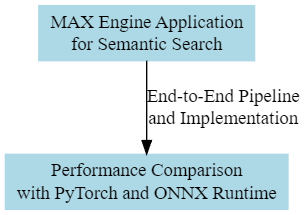
\includegraphics[width=\linewidth]{1.png}}
    \caption{MAX Engine Application and Performance Comparison.}
    \label{fig1}
\end{figure}

\end{itemize}

Figure \ref{fig1} presents the application of MAX Engine for semantic search tasks, particularly in the context of counterfactual statement classification. The workflow encompasses two primary objectives: demonstrating MAX Engine's application for semantic search and comparing its performance against PyTorch and ONNX runtime.
By addressing these objectives, this research contributes to a deeper understanding of how inference-optimized engines like MAX Engine can be leveraged to enhance the efficiency and scalability of semantic search applications in real-world NLP scenarios.

\section {Background Study}
This section delves into the foundations of semantic search, counterfactual statement identification, and the inference frameworks relevant to this research.

\subsection{Semantic Search and its Evolution}
Traditional keyword-based search engines frequently produce irrelevant or insufficient results because they are unable to fully grasp the semantic intricacies of user queries. By comprehending the meaning and intent behind the search query and taking into account elements like context, synonyms, and word relationships, semantic search seeks to get beyond these restrictions [1].
To extract semantic links between words and documents, early approaches to semantic search relied on probabilistic topic models such as Latent Dirichlet Allocation (LDA) [8] and techniques such as Latent Semantic Analysis (LSA) [7]. Nevertheless, these techniques frequently had trouble capturing intricate linguistic phenomena and were not scalable to handle big datasets.
Semantic search underwent a revolution with the introduction of deep learning, specifically with the creation of word embeddings such as Word2Vec [2] and GloVe [8]. Word embeddings use patterns of co-occurrence in huge text corpora to encode semantic connections between words as dense vectors. These embeddings opened the door for more sophisticated sentence and document embedding models and allowed for more precise similarity estimations.

\subsection{Counterfactual Statement Identification}
Counterfactual statements, characterized by their hypothetical and often unrealized nature, pose a unique challenge for NLP tasks [12]. These statements require understanding not only the literal meaning of words but also the implied world knowledge and reasoning about alternative possibilities [3].
Previous approaches to counterfactual identification have explored rule-based methods relying on syntactic patterns and lexical cues [6]. However, these methods often lack robustness and fail to generalize well to diverse linguistic expressions. More recently, machine learning techniques, particularly deep neural networks, have demonstrated promising results in automatically learning complex patterns from labeled data [4],[10].
The goal of this research is to discover counterfactual claims by utilizing the power of semantic similarity, which is derived from pre-trained phrase embeddings. The authors can determine a sentence's probability of falling into the counterfactual class by comparing its embedding with that of known counterfactual and non-counterfactual sentences.

\subsection{Inference Frameworks for NLP}
While it is crucial to develop correct deep learning models, speed and efficiency optimization are frequently needed when deploying these models for real-time inference[11].

\begin{itemize}

    \item \textbf{PyTorch}: PyTorch, a popular deep learning framework, provides flexibility and a wide range of tools for model development and experimentation. However, its eager execution mode may not be optimal for high-performance inference, particularly for large batch sizes.

    \item \textbf{ONNX Runtime}: ONNX Runtime (ORT) offers a cross-platform inference engine optimized for both CPU and GPU execution. It supports models from various frameworks, including PyTorch, allowing for streamlined deployment and improved inference performance.

    \item \textbf{MAX Engine}: MAX Engine is an inference-focused engine designed for maximizing the throughput and minimizing the latency of deep learning models on Intel architectures. It leverages hardware optimizations and efficient memory management techniques to accelerate inference, particularly for batched data.

\end{itemize}

This research benchmarks the performance of these three frameworks PyTorch, ONNX Runtime, and MAX Engine in the context of our semantic search pipeline for counterfactual statement classification.

\section{Methodology}
This section outlines the step-by-step methodology employed in this research, encompassing dataset preparation, embedding generation, vector database integration, classification, and performance evaluation.

\subsection{Dataset Preparation}
The authors utilize the Amazon Multilingual Counterfactual Dataset (AMCD) [4], focusing on the English subset (EN\_train.tsv and EN\_test.tsv for training and testing, respectively). The dataset is loaded and preprocessed using the following steps:

\begin{itemize}
    \item \textbf{Data Loading}: The dataset is loaded into a pandas DataFrame for efficient data manipulation [14].

    \item \textbf{Text Tokenization}: The authors employ the tokenizer associated with the BAAI/bge-base-en-v1.5 model [5] to convert each sentence into a sequence of tokens, suitable for input to the embedding model.
\end{itemize}

\subsection{Sentence Embedding Generation}
To capture the semantic meaning of the sentences, the authors generate sentence embeddings using the pre-trained BAAI/bge-base-en-v1.5 model [5],[16],[17]. For this study, the Hugging Face model hub's ONNX version of the model was used. A standardized format for expressing deep learning models is offered by ONNX (Open Neural Network Exchange), facilitating compatibility between various hardware platforms and frameworks. The ONNX model is loaded using the model. session method.

Steps for generating embeddings:
\begin{itemize}
    \item \textbf{Batching}: Input sentences are divided into batches to optimize processing speed and memory utilization.

    \item \textbf{Model Inference}: Each batch of tokenized sentences is processed by the BAAI/bge-base-en-v1.5 model through maxmodel.execute() to obtain embeddings.

    \item \textbf{CLS Token Extraction}: The [CLS] token embedding, representing the overall sentence, is extracted from the model output.

    \item \textbf{Concatenation}: The [CLS] embeddings from all batches are concatenated into a single matrix, with each row representing a sentence embedding.
\end{itemize}

\subsection{Vector Database Integration}
For efficient storage and querying of sentence embeddings, the authors integrate the system with ChromaDB, an open-source vector database designed for machine learning applications [13]. Interaction with ChromaDB is managed using its Python client library.

Steps include: 

\begin{itemize}
    \item \textbf{Collection Creation}: A collection named \texttt{counterfactual\_collection} is created in ChromaDB, using cosine similarity as the distance metric for nearest neighbor searches. 

    \item \textbf{Data Insertion}: Sentence embeddings, along with their corresponding sentences and labels, are inserted into the ChromaDB collection.
\end{itemize}

\subsubsection{Classification and Evaluation}
For classifying a given query sentence, the process involves:

\begin{itemize}
    \item \textbf{Query Embedding} : The query sentence is tokenized and processed by the BAAI/bge-base-en-v1.5 model to obtain its embedding.
    \item \textbf{Similarity Search} : The query embedding is used to retrieve the top k similar sentences from the ChromaDB collection based on cosine similarity.
    \item \textbf{Counterfactual Probability} :  The \texttt{is\_counterfactual} labels of the k nearest neighbors are averaged to determine the probability of the query being counterfactual.
    \item \textbf{Prediction} : The query sentence is classified as counterfactual if the calculated counterfactual probability exceeds a predefined threshold; otherwise, it is classified as non-counterfactual.
\end{itemize}
Effectiveness is evaluated using standard classification metrics on the test set:
\begin{itemize}
    \item \textbf{Accuracy} : The ratio of correctly classified sentences to the total number of sentences.
    \item \textbf{F1-Score} : The harmonic mean of precision and recall.
    \item \textbf{Precision} : The ratio of correctly classified counterfactual sentences to the total number of sentences classified as counterfactual.
    \item \textbf{Recall} : The ratio of correctly classified counterfactual sentences to the total number of actual counterfactual sentences.
\end{itemize}

\subsection{Performance Benchmarking}
The time required to generate embeddings for the entire dataset using each framework under various batch size configurations is measured to compare the inference speed of MAX Engine against PyTorch and ONNX Runtime.

Steps include:
\begin{itemize}
    \item \textbf{Variation in Batch Size} : A range of batch sizes, from small (1, 2, 4, 8, 16, 32) to large (64, 128, 256, 512, 1024, 2048, 4096) values, are used to assess the scalability of performance.
    \item \textbf{Time Measurement} : The average time required to process a batch of sentences is determined for each batch size, considering numerous iterations to account for runtime variations.
    \item \textbf{Hardware} : Benchmarking is performed on a GitHub Codespace instance with 4 CPU cores and 16 GB RAM, ensuring a consistent and controlled hardware environment for fair comparison.
\end{itemize}

\begin{figure}[h]
    \centerline{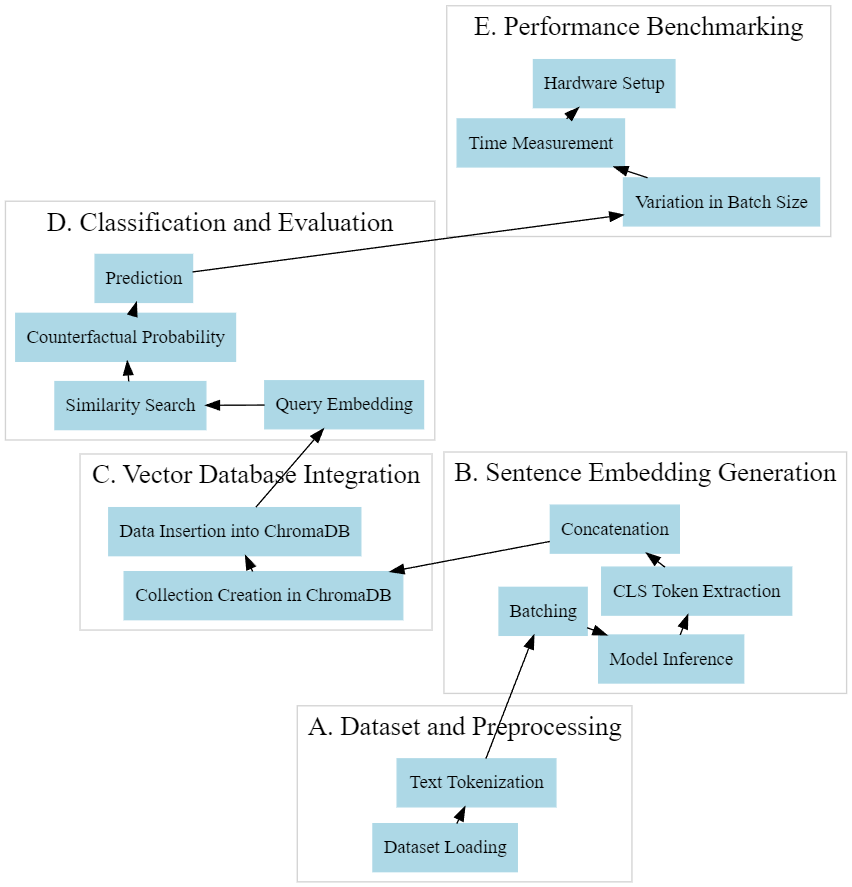
\includegraphics[width=\linewidth]{2.png}}
    \caption{Data Preprocessing to Performance Benchmarking.}
    \label{fig2}
\end{figure}

Figure \ref{fig2} provides an overview of the end-to-end process from data preprocessing to performance benchmarking in the context of counterfactual statement classification using MAX Engine. The workflow begins with dataset preprocessing, including data loading and text tokenization, followed by sentence embedding generation using MAX Engine.
By examining runtime results across various batch sizes, the authors gain insights into the efficiency and scalability of MAX Engine in comparison to PyTorch and ONNX Runtime.

\section{Results and Discussion}
This section presents the findings of our experiments, analyzing both the classification performance of our semantic search-based approach for counterfactual statement identification and the inference speed comparison between MAX Engine, PyTorch, and ONNX Runtime.

\subsection{Classification Performance}
The authors evaluated our system's ability to distinguish between counterfactual and non-counterfactual statements using the metrics outlined in Section 3.4. The results, obtained on the AMCD English test set with a threshold of 0.5 for counterfactual probability, are presented below in \ref{tab:metrics}:

\captionsetup[table]{skip=10pt}
\begin{table}[H]
    \centering
    \begin{tabular}{|l|l|}
    \hline
    \textbf{Metrics} & \textbf{Score} \\
    \hline
    Accuracy & 0.88 \\
    \hline
    F1-Score & 0.64 \\
    \hline
    Precision & 0.75 \\
    \hline
    Recall & 0.56 \\
    \hline
    \end{tabular}
    \caption{Performance of the Classification}
    \label{tab:metrics}
\end{table}

These results demonstrate the effectiveness of leveraging semantic similarity for counterfactual statement identification. The relatively high accuracy suggests that sentences with similar semantic content tend to share the same counterfactual characteristic. However, the moderate F1-score, particularly the lower recall, highlights areas for potential improvement. The recall value indicates that our system might misclassify some counterfactual statements, suggesting the need to explore more sophisticated methods for capturing subtle linguistic cues associated with counterfactuality.

\subsection{Inference Speed Comparison}
Figure \ref{fig3} and Figure \ref{fig4} depict the inference speed comparison between MAX Engine, PyTorch, and ONNX Runtime, measured in terms of average batch processing time (seconds) across varying batch sizes.

\begin{itemize}
    \item \textbf{Smaller Batch Sizes (1-32)}
    \begin{figure}[H]
        \centerline{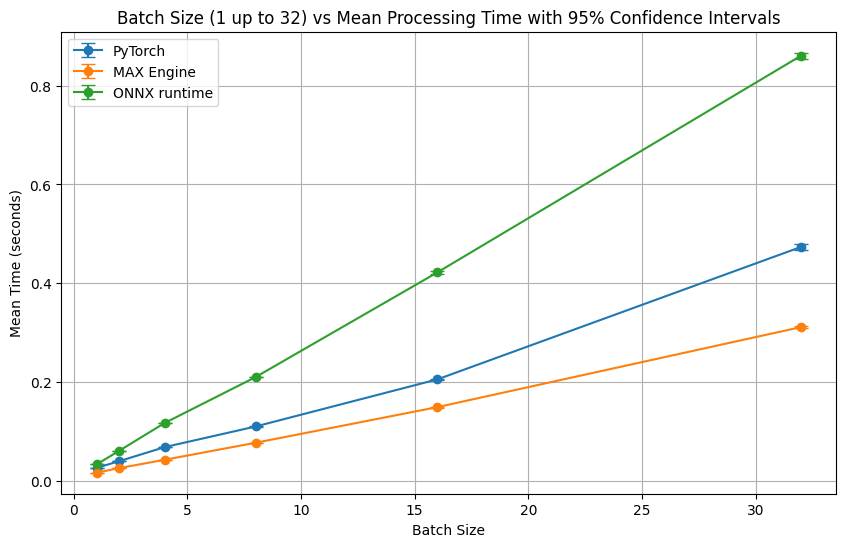
\includegraphics[width=\linewidth]{3.png}}
        \caption{Bar chart comparing inference time for smaller batch sizes.}
        \label{fig3}
    \end{figure}
    For smaller batch sizes, MAX Engine consistently outperforms both PyTorch and ONNX Runtime, demonstrating up to 1.6 times faster inference compared to PyTorch and up to 2.8 times faster than ONNX Runtime. This speedup can be attributed to MAX Engine's focus on optimizing inference workloads for Intel architectures, allowing it to efficiently handle smaller batches with minimal overhead.

    \item \textbf{Larger Batch Sizes (64-4096)}
    \begin{figure}[H]
        \centerline{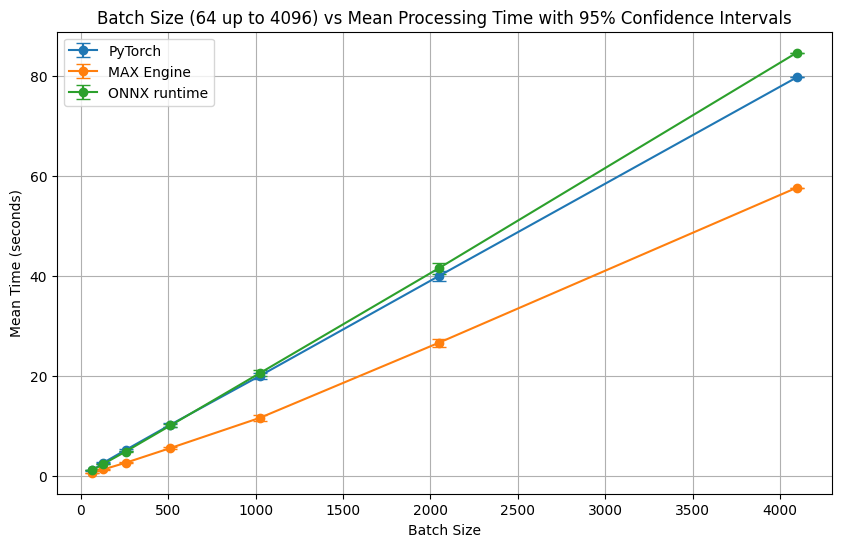
\includegraphics[width=\linewidth]{4.png}}
        \caption{ Line chart comparing inference time for larger batch sizes.}
        \label{fig4}
    \end{figure}
    As the batch size increases, the performance difference between the frameworks becomes more pronounced. MAX Engine exhibits superior scalability, maintaining a significant speed advantage over PyTorch and ONNX Runtime, especially as batch size grows. This scalability is crucial for real-world NLP applications dealing with large volumes of data, as it directly translates to faster processing times and improved resource utilization.
\end{itemize}

\subsection{Assess Test Accuracy, F1-score, Precision and Recall}
The authors assess the model using standard metrics on a test dataset. The F1-score strikes a compromise between precision and recall; precision gauges the model's exactness, while recall evaluates its completeness. Accuracy gives an overall impression of performance [20].
\begin{figure}[H]
    \centerline{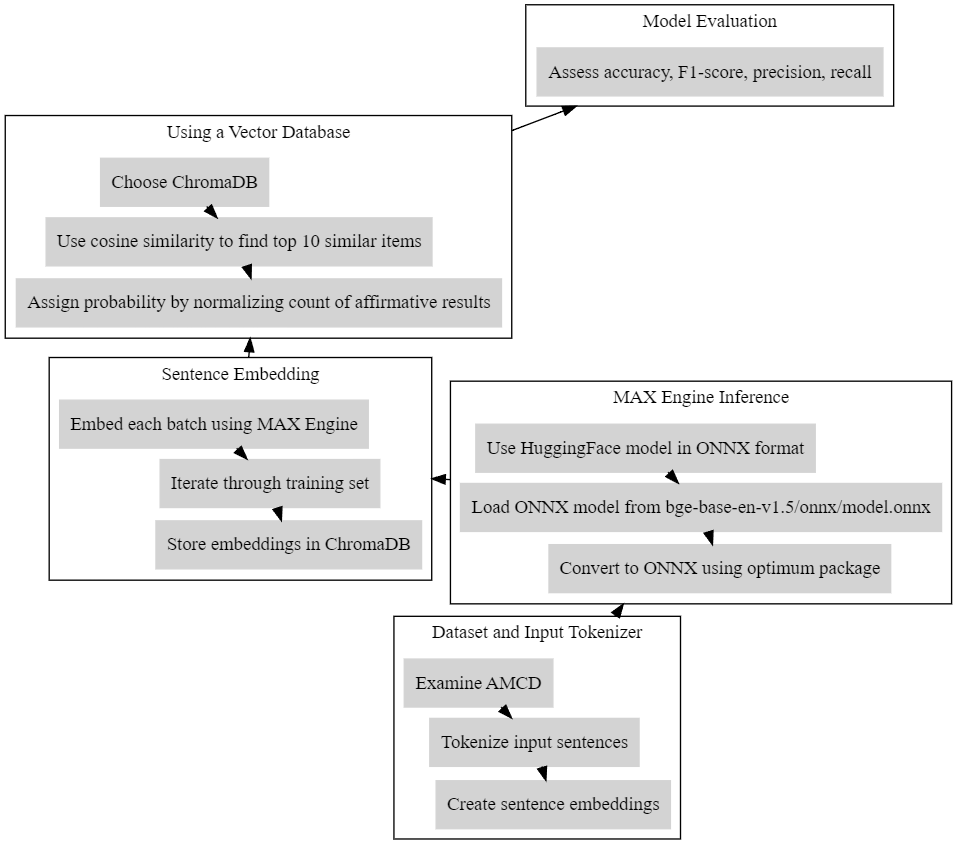
\includegraphics[width=\linewidth]{5.png}}
    \caption{Workflow for Counterfactual Statement Classification Using MAX Engine and ChromaDB.}
    \label{fig5}
\end{figure}
Figure \ref{fig5} illustrates the workflow for counterfactual statement classification using MAX Engine and ChromaDB. The process begins with dataset preprocessing, where the Amazon Multilingual Counterfactual Dataset (AMCD) is loaded and tokenized. These tokens are then fed into the BAAI/bge-base-en-v1.5 model to generate sentence embeddings. These embeddings are stored in ChromaDB, a vector database, for efficient storage and querying.

\subsection{Comparing MAX Engine performance against PyTorch eager and ONNX}
Recall that the authors used a batch size of 128 to process the sentence embeddings to compute them all quickly. In situations involving large amounts of data, batching is crucial for maximizing resource efficiency and processing speed. Thus, our goal is to evaluate how well MAX Engine performs about PyTorch and ONNX runtime for different batch sizes to determine how effective each tool is at managing batched data. The authors carefully chose a range of batch sizes and, for improved visibility, separated them into two groups of

\begin{itemize}
    \item textbf{smaller batch sizes}: 1 up to 32
    \item textbf{larger batch sizes}: 64 up to 4096
\end{itemize}

\begin{figure}[H]
    \centerline{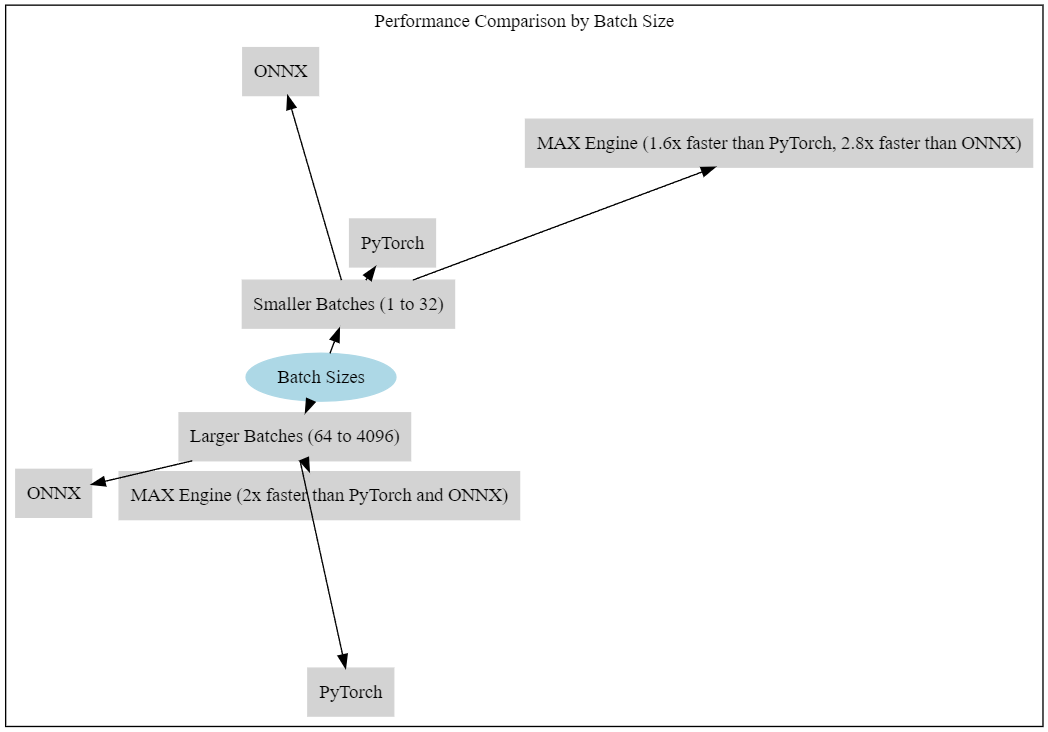
\includegraphics[width=\linewidth]{6.png}}
    \caption{Comparing MAX Engine Performance Against PyTorch and ONNX .}
    \label{fig6}
\end{figure}

Fig. \ref{fig6} provides a comparative analysis of MAX Engine performance against PyTorch and ONNX runtime in terms of inference speed across various batch sizes. The x-axis represents different batch sizes ranging from small to large values, while the y-axis indicates the average time required to process a batch of sentences.     
These large arrays let us see how well each framework performs under various load scenarios in terms of scalability and efficiency. Each batch size's runtime is assessed, providing a clear picture of how each framework manages different data quantities. In resource-intensive scenarios, like working with enormous datasets, this evaluation is essential for developers and engineers to make well-informed judgments regarding the tools and frameworks best suited for their particular NLP jobs. Runtime measurements were performed on a GitHub Codespace 4 Core CPU \& 16 GB instance for completeness.
Now, the authors plot the performance of each model using PyTorch, ONNX, and MAX Engine separately. According to this examination of the first graph, MAX Engine can perform batch inference up to 2.8 times quicker than ONNX runtime and up to 1.6 times faster than PyTorch for smaller batch sizes (1 to 32).

\begin{figure}[H]
    \centerline{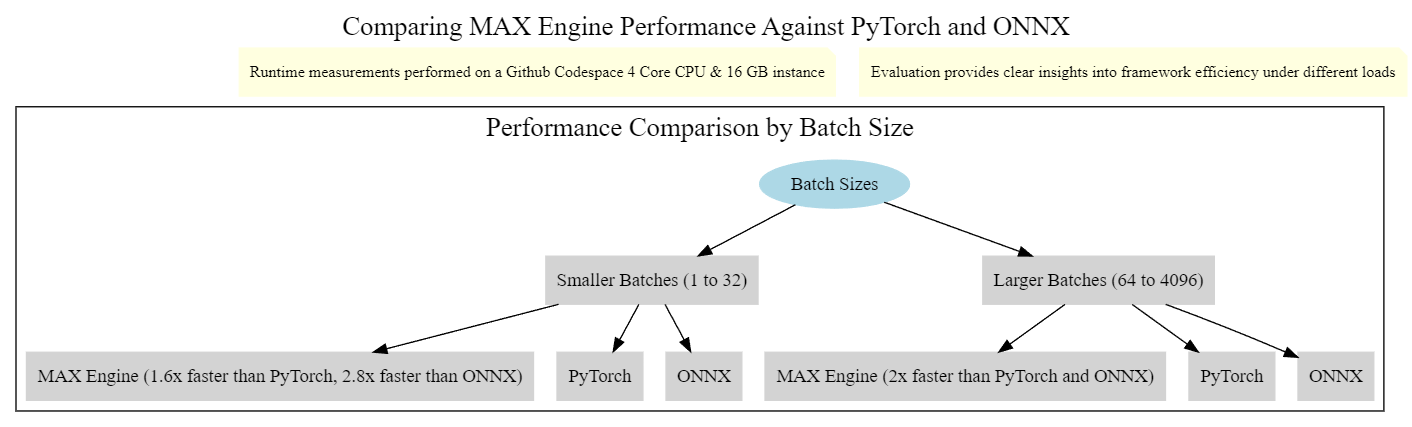
\includegraphics[width=\linewidth]{7.png}}
    \caption{Performance Comparison of MAX Engine, PyTorch, and ONNX.}
    \label{fig7}
\end{figure}

Fig. \ref{fig7} depicts a performance comparison among MAX Engine, PyTorch, and ONNX across various evaluation metrics. Each bar represents the average performance of the respective framework in terms of accuracy, F1-score, precision, and recall.
MAX Engine may run up to two times quicker than PyTorch and ONNX runtime for bigger batch sizes (64 up to 4096), respectively. This demonstrates how well the MAX Engine can handle demanding data processing jobs. Additionally, MAX Engine can run up to two times faster than PyTorch and ONNX runtime for bigger batch sizes (64 up to 4096). 
This demonstrates how well the MAX Engine can handle demanding data processing tasks.

\section{Conclusion}
This research demonstrates the effectiveness of using the MAX Engine to accelerate semantic search tasks, particularly for classifying counterfactual statements. By leveraging the BAAI/bge-base-en-v1.5 sentence embedding model and the ChromaDB vector database, the authors developed an end-to-end pipeline capable of effectively distinguishing between counterfactual and non-counterfactual statements. Our results highlight the significant speed advantages offered by MAX Engine compared to PyTorch and ONNX Runtime, especially for larger batch sizes typical in real-world applications. The study shows that using semantic similarity for counterfactual identification with pre-trained embeddings can yield promising results. MAX Engine consistently delivers superior inference speed, outperforming both PyTorch and ONNX Runtime across all tested batch sizes, which significantly reduces inference time and enhances processing throughput. This superior scalability makes MAX Engine a compelling choice for deploying NLP models in production environments that require real-time or near real-time processing of large datasets. The findings of this research have significant implications for developers and researchers working on NLP applications involving semantic search, text classification, and other tasks requiring efficient inference. By adopting inference-optimized engines like MAX Engine, developers can significantly accelerate inference, optimize resource utilization, and enhance user experience with faster response times and improved performance. Future research could explore fine-tuning the sentence embedding model for specific domains or tasks to further enhance accuracy[18]. Experimenting with alternative vector database technologies and configurations may help identify optimal solutions for managing and querying large-scale embedding datasets. Additionally, applying this semantic search framework to other NLP tasks, such as question answering, text summarization, and information retrieval, could unlock new opportunities for developing robust, scalable, and efficient NLP applications capable of handling the increasing volume and complexity of textual data.



\begin{thebibliography}{00}
\bibitem{b1} Schütze, Hinrich, Christopher D. Manning, and Prabhakar Raghavan. Introduction to information retrieval. Vol. 39. Cambridge: Cambridge University Press, 2008.
\bibitem{b2} Mikolov, Tomas, et al. "Distributed representations of words and phrases and their compositionality." Advances in neural information processing systems 26 (2013).
\bibitem{b3} GOODMAN, N. "THE PROBLEM OF COUNTERFACTUAL CONDITIONALS." (2001): 81-98.
\bibitem{b4} O'Neill, James, et al. "I Wish I Would Have Loved This One, But I Didn't--A Multilingual Dataset for Counterfactual Detection in Product Reviews." arXiv preprint arXiv:2104.06893 (2021).
\bibitem{b5} Xiao, Shitao, et al. "C-Pack: Packaged Resources To Advance General Chinese Embedding." 2023, arXiv, doi:2309.07597.
\bibitem{b6} Deerwester, Scott, et al. "Indexing by latent semantic analysis." Journal of the American society for information science 41.6 (1990): 391-407.
\bibitem{b7} Blei, David M., Andrew Y. Ng, and Michael I. Jordan. "Latent dirichlet allocation." Journal of machine Learning research 3.Jan (2003): 993-1022.
\bibitem{b8} Pennington, Jeffrey, Richard Socher, and Christopher D. Manning. "Glove: Global vectors for word representation." Proceedings of the 2014 conference on empirical methods in natural language processing (EMNLP). 2014.
\bibitem{b9} Son, Youngseo, et al. "Recognizing counterfactual thinking in social media texts." Proceedings of the 55th Annual Meeting of the Association for Computational Linguistics (Volume 2: Short Papers). 2017.
\bibitem{b10} Loper, Edward, and Steven Bird. "NLTK: The Natural Language Toolkit." Proceedings of the ACL-02 Workshop on Effective tools and methodologies for teaching natural language processing and computational linguistics-Volume 1. Association for Computational Linguistics, 2002.
\bibitem{b11} Devlin, Jacob, et al. "BERT: Pre-training of Deep Bidirectional Transformers for Language Understanding." arXiv preprint arXiv:1810.04805 (2018).
\bibitem{b12} Vaswani, Ashish, et al. "Attention is All You Need." Advances in Neural Information Processing Systems 30 (NIPS 2017).
\bibitem{b13} Peters, Matthew E., et al. "Deep contextualized word representations." Proceedings of NAACL-HLT 2018.
\bibitem{b14} Rajpurkar, Pranav, et al. "SQuAD: 100,000+ questions for machine comprehension of text." Proceedings of the 2016 Conference on Empirical Methods in Natural Language Processing. 2016.
\bibitem{b15} Brown, Tom B., et al. "Language models are few-shot learners." Advances in Neural Information Processing Systems 33 (NIPS 2020).
\bibitem{b16} Liu, Yinhan, et al. "Roberta: A robustly optimized bert pretraining approach." arXiv preprint arXiv:1907.11692 (2019).
\bibitem{b17} Lewis, Mike, et al. "BART: Denoising sequence-to-sequence pre-training for natural language generation, translation, and comprehension." Proceedings of the 58th Annual Meeting of the Association for Computational Linguistics. 2020.
\bibitem{b18} Lewis, Mike, et al. "BART: Denoising sequence-to-sequence pre-training for natural language generation, translation, and comprehension." Proceedings of the 58th Annual Meeting of the Association for Computational Linguistics. 2020.
\bibitem{b19} Radford, Alec, et al. "Language models are unsupervised multitask learners." OpenAI Blog 1.8 (2019).
\bibitem{b20} Le, Quoc V., and Tomas Mikolov. "Distributed representations of sentences and documents." Proceedings of the 31st International Conference on Machine Learning (ICML-14). 2014.
\end{thebibliography}

\end{document}
